\documentclass[10pt,letterpaper,xcolor=dvipsnames]{article}

%\usepackage[colorlinks=true,linkcolor=blue]{hyperref}
\usepackage{amssymb}
\usepackage{linguex}
\usepackage{verbatim,enumerate,multirow}
\usepackage{xcolor}
%\usepackage{floatflt}

%% Pdf rendering - uncomment for html 
%\def\pgfsysdriver{pgfsys-tex4ht.def}          

\usepackage{tikz}
\usepackage{xstring}

\def\pyramid{(-1.5,1) -- (1.5,1) -- (0,-1) -- (-1.5,1);}
\def\levels{-0.75,-0.5,...,1}
\def\props{-1,-0.6,...,2.4}

\def\xodd{-1.5,-0.5,...,2.5}
\def\xeven{-2,-1,...,2}
\def\yodd{1.25,0.25,-0.75,-1.75}
\def\yeven{1.75,0.75,-0.25,-1.25}

\tikzstyle{every node}=[font=\tiny]

\begin{document}

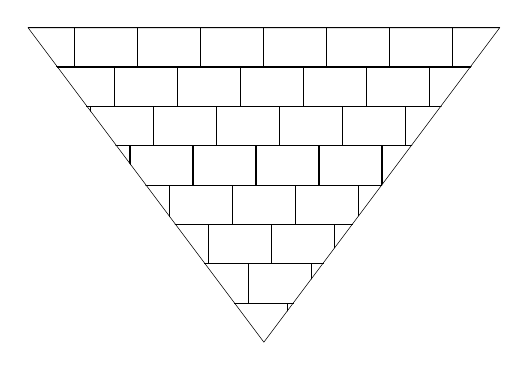
\begin{tikzpicture}

  \begin{scope}[scale=2]
  \clip \pyramid;
  \foreach \y [count=\yi] in \levels
    \foreach \x [count=\xi] in \props
    {
      \draw (-1.5,\y) -- (1.5,\y);
      \draw (\x-\y,\y) -- (\x-\y,\y-0.25);
      \node at (\x,\y) (\yi\xi) {};
    }
  \draw \pyramid;
  \end{scope}

\begin{comment}
  \begin{scope}
  \node at (3,0.5) (p) {Propositions};
  \node at (2.75,0) (s) {Support relation};
  \node at (2.5,-0.5) (a) {Axioms};
    \draw[->] (p.north west) to[bend right] (54.north);
    \draw[-] (s.west) to (47.center);
    \draw[->] (47.center) to[bend right] (46.north);
    \draw[->] (47.center) to[bend left] (46.south);
    \draw[->] (a.south west) to[bend left] (14.south);
  \end{scope}
\end{comment}

\end{tikzpicture}

\vspace{2cm}

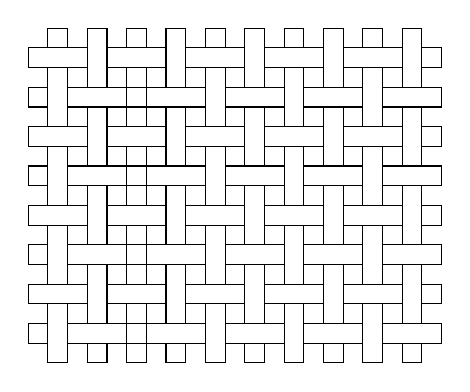
\begin{tikzpicture}

\begin{scope}
  \foreach \x in \xeven {
      \draw (\x,1.75) -- (\x,2) -- (\x+0.25,2) -- (\x+0.25,1.75);
      \draw (\x,0.75) -- (\x,1.5) (\x+0.25,0.75) -- (\x+0.25,1.5);
      \draw (\x,-0.25) -- (\x,0.5) (\x+0.25,-0.25) -- (\x+0.25,0.5);
      \draw (\x,-1.25) -- (\x,-0.5) (\x+0.25,-1.25) -- (\x+0.25,-0.5);
      \draw (\x,-1.5) -- (\x,-2.25) -- (\x+0.25,-2.25) -- (\x+0.25,-1.5);
  }
  \foreach \x in \xodd {
    \draw (\x,1.25) -- (\x,2) -- (\x+0.25,2) -- (\x+0.25,1.25);
      \draw (\x,1) -- (\x,0.25) (\x+0.25,1) -- (\x+0.25,0.25);
      \draw (\x,0) -- (\x,-0.75) (\x+0.25,0) -- (\x+0.25,-0.75);
      \draw (\x,-1) -- (\x,-1.75) (\x+0.25,-1) -- (\x+0.25,-1.75);
    \draw (\x,-2) -- (\x,-2.25) -- (\x+0.25,-2.25) -- (\x+0.25,-2);
  }

  \foreach \y in \yeven {
      \draw (-1.5,\y) -- (-2.25,\y) -- (-2.25,\y-0.25) -- (-1.5,\y-0.25);
      \draw (-1.25,\y) -- (-0.5,\y) (-0.5,\y-0.25) -- (-1.25,\y-0.25);
      \draw (-0.25,\y) -- (0.5,\y) (0.5,\y-0.25) -- (-0.25,\y-0.25);
      \draw (0.75,\y) -- (1.5,\y) (1.5,\y-0.25) -- (0.75,\y-0.25);
      \draw (1.75,\y) -- (2.5,\y) (2.5,\y-0.25) -- (1.75,\y-0.25);
      \draw (2.75,\y) -- (3,\y) -- (3,\y-0.25) -- (2.75,\y-0.25);
  }

  \foreach \y in \yodd {
      \draw (-2,\y) -- (-2.25,\y) -- (-2.25,\y-0.25) -- (-2,\y-0.25);
      \draw (-1.75,\y) -- (0,\y) (0,\y-0.25) -- (-1.75,\y-0.25);
      \draw (0.25,\y) -- (1,\y) (0.25,\y-0.25) -- (1,\y-0.25);
      \draw (2,\y) -- (1.25,\y) (1.25,\y-0.25) -- (2,\y-0.25);
      \draw (2.25,\y) -- (3,\y) -- (3,\y-0.25) -- (2.25,\y-0.25);
  }

\end{scope}

\end{tikzpicture}

\end{document}
